\section{Data Link Laget}
Data Link Laget (DLL) blev indført for at opnå pålidelighed af modtagne beskeder. Derudover indeholder DLL en konverterings klasse, \texttt{ToneKonvertering}, hvis formål er at konvertere dataen til et format som det fysiske lag kan forstå. Dette kræver at dataen før \texttt{ToneKonvertering} går op i 3, da hver tone tilsvarer 3 bit.

\subsection{Teori}
CRC står for Cyklisk Redundant Check, og bruges til fejldetektering. Formålet med fejldetektering er at gøre det muligt for modtageren at afgøre om et datagram, sendt gennem en støjet kanal, er blevet korrupt. For at gøre dette konstruerer senderen en checksum og tilføjer denne på datagrammet.
\newline
Modtageren er i stand til at bruge CRC til at beregne checksum af det modtagne datagram og sammenligne denne med den vedlagte checksum for at se, om datagrammet er blevet modtaget korrekt.
\newline
CRC er baseret på polynomiel aritmetik, som primært består af beregning af resten når et polynomium divideres med et andet polynomium. Et eksempel kan ses i figur \ref{fig:poly}.
\begin{figure}[ht]
	\centering
	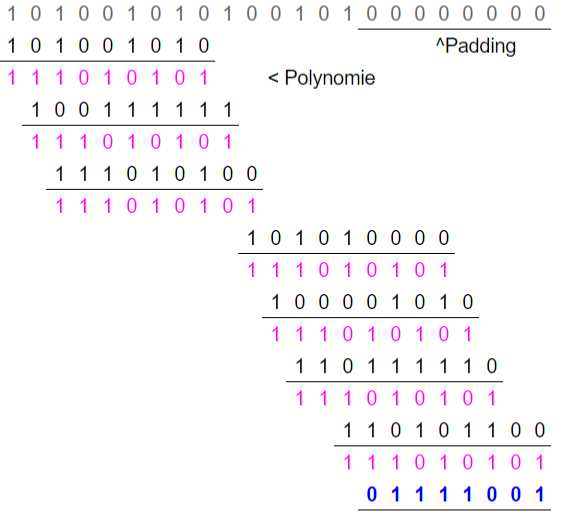
\includegraphics[width=10cm,height=20cm,keepaspectratio]{pictures/Poly.png}
	\caption{Eksempel på polynomiel division}
	\label{fig:poly}
\end{figure}
\newline
Her er grå den originale besked, pink er polynomiet og blå er checksum.

\subsection{Implementering}
For at opnå pålidelig modtagelse af beskeder, blev et CRC indført. Dette gør at alle sendte beskeder skal indeholde et CRC, som bliver beregnet ud fra den originale besked.
\newline
Når denne besked modtages af en anden applikation, skal det samme CRC kunne udregnes og sammenlignes med det medfølgende CRC check. Hvis disse 2 checks er identiske, kan beskeden accepteres som korrekt.
\hfill \break

For at oprette et CRC check, skal man først definere størrelsen af det CRC check man vil benytte. Originalt i applikationen var fejlsikring en stor prioritet, og beskeder blev sendt i en stor pakke, så et stort CRC-32 blev valgt, for at kunne finde flest mulige fejl. Dette kan udføres vha. polynomiel division.
\newline
For at benytte CRC-32, blev en tabel med 256 værdier oprettet på baggrund af en smart metode at implementere CRC checket. Dette tillader koden at lave den polynomielle aritmetik på forhånd, uden at vide hvilken bitstreng den modtager. Hver af disse værdier i tabellen tilsvarer CRC-32 checksummen for et 8 bits udtryk ($2^8 = 256$). Koden skal dermed hente dele af bitstrengen, og slå op i tabellen hvad hver eneste par af 8 bit tilsvarer. Dette udføres indtil der kun er 32 bits tilbage, og dette tilsvarer checksummen for beskeden.
Denne løsning var præget af at skulle virke hurtigt, og var derfor limiteret af forskellige faktorer, såsom at CRC checken kun virker på udtryk der er længere end 32 bits. Derudover var den lavet overskuelig ved brug af hexadecimale tal, både i tabellen og i den resulterende checksum, som krævede ekstra konvertering tilbage til bitstreng.
\newline
Denne checksum bliver sendt sammen med beskeden, i en trailer, for at tillade modtageren at udføre samme CRC check, og verificere at beskeden er modtaget korrekt.
\newline
Denne checksum tilføjede 32 bits til datagrammet, og skabte en problemstilling i forhold til at sende dataen videre via \texttt{ToneKonvertering}, da det samlede datagram ikke gik op i 3 længere.
\newline
I \texttt{ToneKonvertering} skulle bitstrengen kunne opdeles i dele af 3 bits hver. Denne problemstilling bliver løst, ved at stuffe beskeden med ekstra bits. For at gøre det nemmere at fjerne stuffing, bliver der altid tilføjet stuffing, selv om beskeden originalt kunne opdeles. Ved at gøre dette slipper man uden om spørgsmålet, om der skal fjernes stuffing, da der altid skal fjernes stuffing. Stuffing bliver udført ved at tilføje 1 til 3 bits alt efter længden af beskedens bits. Mængden af stuffing, der skal pålægges beskeden, kan findes ved at tage modulus-3 af beskedens længde. Denne stuffing bestod af først et 1-tal, og dernæst 0’er indtil kravet om længden af stuffing er opfyldt. Dermed kan modtager siden identificere det 1-tal der forekommer først i traileren på datagrammet, og fjerne indtil denne.
\newline
Modtagersiden skulle dernæst kunne confirmere at beskedens checksum er korrekt, og derfor bliver datagrammer ved modtagelse splittet ud i besked data, og checksum. Den samme checksum skal kunne udregnes fra den modtagne besked, ellers er der sket en fejl i transmission af beskeden.
\newline
Når transportlaget blev implementeret, blev meget mindre pakker sendt imellem applikationer, og CRC-32 checket viste sig at fylde mere end de sendte beskeder, og limitationer med længden af bitstrengen skabte ugyldige beskeder. Derfor blev CRC checket reduceret til et CRC-8. Dette skabte en kortere checksum, som dermed formindsker behovet for antallet af toner der skal sendes af applikationen.
\newline
Dette blev udført kodemæssigt med et 8 bits CRC check, som er en simpel XOR operation på beskeden. For at sikre håndtering af bits, snarere end integers, skal bitset dataholdere benyttes.
\newline
Det valgte polynomie er: $x8 + x7 + x6 + x4 + x2 + 1$, hvilket tilsvarer 111010101 i bits. Dette polynomie vil finde alle single-bit errors, og uneven-bit errors.
Kodemæssigt bliver der først padded med 8 bits på beskeden. Dette bliver i slutningen af den polynomiale divison til checksummen. Dernæst bliver bits fra datagrammet, eller beskeden, taget ud, tilsvarende til længden af bits i polynomiet og dette bliver XOR’et med polynomiet. Dette gøres indtil der kun er bits i checksummen.
\hfill \break

\texttt{ToneKonvertering}s klassen fungerer som en basal oversætter, der transformerer datagrammet fra en bitstreng til en sekvens af lyde, som det fysiske lag kan behandle.
\newline
Der blev stødt ind i en problemstilling, der omhandlede hvor mange ens toner, der blev modtaget i træk. For at tage hensyn til dette, blev der defineret et flag. Dette flag bliver indsat i mellem to ens toner. Dette medførte at optager klassen, \texttt{MyRecorder}, ikke behøver synkronisering, men i stedet er i stand til at finde, når en ny tone modtages. Derudover kræver konverteringen i denne klasse, at antallet af bits kan gå op i 3. Dette tager stuffingen i DLL hensyn til.
\hfill \break

Der ses på 3 bits, som hver oversættes i forhold til deres værdi i bits, til en bestemt tone.
\newline
Tone 0 defineres som bitværdi 000, mens tone 7 defineres som bitværdi 111. Dette bliver gemt i en vektor, som indeholder værdier der tilsvarer toner.
\newline
Da der der ikke kan vides hvor mange toner der kommer af gangen, defineres 8 (DTMF: 7) som en tone flag. Hvis der er behov for at afspille to ens toner afspilles efter hinanden, bliver dette tone flag benyttet.
\newline
Til det fysiske lag defineres et start flag og et slut flag, som henholdsvis tilsvarer tone 14(DTMF: \#) og tone 15(DTMF: d), da dette gør det nemmere for \texttt{MyRecoder} klassen at optage.
\newline
 Al denne information indsættes i en vektor, som videre benyttes af andre klasser.